\section{openHAB}
\label{sec:openhab}
    Neben der so eben erläuterten Home Assistant Plattform zählt ebenso die openHAB Plattform als bekannt und 
    in der Anwendung populär. Der \ac{OPENHAB} ist eine Plattform, bei der es sich um eine 
    Softwarelösung handelt, die auf Basis der Programmiersprache Java aufgebaut ist. Die Software steht unter 
    der Eclipse Public License und fällt daher unter die Rubrik der Open-Source Software. Durch die Verwendung 
    von Java ist die Anwendung betriebssystemunabhängig und kann auf beliebigen Betriebssystemen laufen. 
    Ähnlich zu der vorgestellten Home Assistant Software, bietet openHAB ebenso User Interfaces die durch 
    den Webbrowser, Android- und iOS-Geräte unterstützt werden. 
    \\
    \linebreak
    In Kombination mit Java wird bei openHAB das \ac{OSGI}-Framework für die Modularität der Software verwendet. Mit Apache 
    Karaf wird ein Container bereitgestellt, der mit Eclipse Equinox als \acs{OSGI} Laufzeitumgebung agiert. Als 
    \acs{HTTP}-Server ist Jetty in Gebrauch. Die einzelnen Frameworks werden nicht im Detail erläutert, lediglich die für das 
    Verständnis des Konzeptes notwendigen.
    \\
    \linebreak
    Mit openHAB wird eine hochmodulare Software zur Verfügung gestellt, die durch sogenannte \textit{Add-ons} erweitert 
    werden kann. Durch diese wird der Plattform eine breite Palette an Funktionen geboten. Physische Geräte können in 
    großer Anzahl mit der Plattform interagieren und verknüpft werden.\footnote{Einleitung zu openHAB. \url{https://www.openhab.org/docs/} Abgerufen am 25.04.2022}

    \subsection*{Historie}
    \label{sec:historyoHAB}
    %TBD...

\subsection{Konzept und Architektur}
%\subsection{Architektur}
    Die Steuerungsplattform openHAB bietet vergleichbar zu Home Assistant die Möglichkeit der multifunktionalen Verknüpfung von 
    Geräten und Protokollen. An dieser Stelle werden ebenso mehrere Konzepte verwendet, die die Vereinheitlichung der Plattform 
    verstärkt. Die Konzepte der openHab Software sind in drei größere Rubriken aufgeteilt, die sich wie folgt zusammensetzen:
    \\
    \linebreak
    Die erste Rubrik sind die Dinge (Things), diese sind die Entitäten, die als physische Komponente zu einem System hinzugefügt 
    und viele Funktionalitäten als eines bereitstellen kann. Hierbei ist zu berücksichtigen, dass die sogenannten Dinge nicht 
    immer Geräte sein müssen, diese können auch andere überschaubare Informationsquellen, andere Webdienste und Funktionalitäten 
    darstellen. Aus Sicht des Benutzers sind sie für den Einrichtungs- und Konfigurationsprozess relevant, für den Betrieb 
    jedoch potentiell zu vernachlässigen. Dinge können Konfigurationseigenschaften haben, die optional oder obligatorisch sein 
    können. Solche Eigenschaften können grundlegende Informationen wie eine IP-Adresse, ein Zugriffstoken für einen Webdienst 
    oder eine gerätespezifische Konfiguration sein, die sein Verhalten ändert \cite{openHAB-article}. Mit dem Konzept der Dinge 
    kommen zwei Unterkategorien einher:
    \begin{itemize}
        \item Kanäle (Channels): Jedes Gerät, bzw. Ding stellt Kanäle bereit, mit denen die jeweiligen Funktionen abgebildet werden. 
        An der Stelle an der das physische Gerät angebunden ist, ist der Kanal eine konkrete Funktion dieser Entität. Beispielsweise 
        kann eine Glühbirne einen Kanal für die Farbtemperatur und einen für den Farbwert besitzen. Diese stellen beide die 
        Funktionalität der einen physischen Glühbirne für das System bereit. Grundlegend sind Kanäle mit Elementen verknüpft, mit denen 
        die virtuelle und physische Ebene verbunden wird. Ab dem Zeitpunkt, sobald eine Verbindung hergestellt wird, reagiert ein Ding 
        auf Ereignisse, die für ein Element transferiert werden. Bedingung dafür ist die Verknüpfung zu einem Kanal. Auf der anderen 
        Seite werden aktiv Ereignisse für Objekte gesendet, die mit Kanälen des Dings verknüpft sind \cite{openHAB-article}.
        \item Brücken (Bridges): Die Brücke ist eine besondere Art von Ding. Diese müssen dem System hinzugefügt werden, damit der 
        Zugriff auf andere Dinge ermöglicht wird, bzw. erhalten bleibt. Ein IP-Gateway für Hausautomationssysteme, welches nicht 
        IP-basiert funktioniert, ist eine typisches Beispiel für so eine Brücke.
    \end{itemize}
    An zweiter Stelle stehen die Artikel (Items). Diese Elemente stellen Funktionen dar, die direkt von der Anwendung verwendet 
    werden. Darunter zählen hauptsächlich die Automatisierungslogik oder auch Benutzeroberflächen. Durch Ereignisse werden die 
    Elemente verwendet, da diese einen Zustand besitzen. 
    \begin{figure}[hbt!]
        \centering
        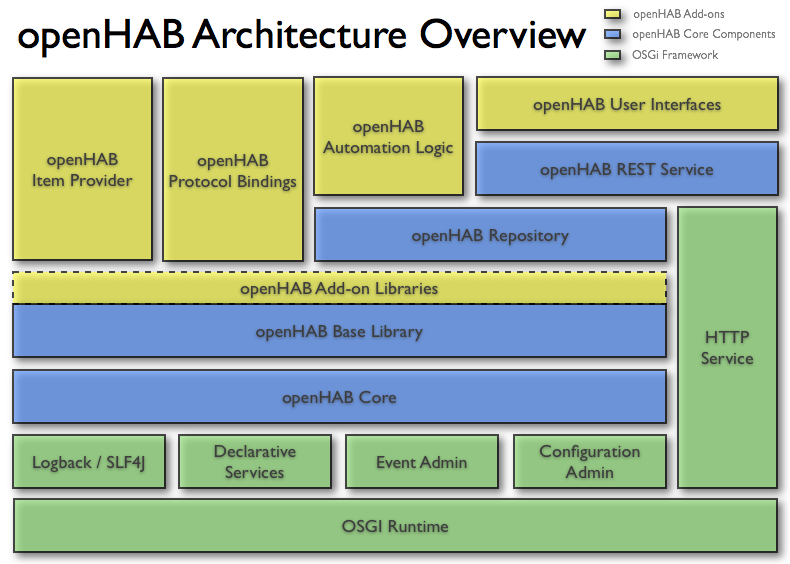
\includegraphics[width=12cm,height=12cm,keepaspectratio]{images/openhab-architecture.png}
        \caption{Architektur der openHAB Plattform \cite{openHAB-architecture2018}}
        \label{fig:architectureopenHAB}
    \end{figure}




\subsection{Ziele und Schwerpunkte}
\subsection{Stärken und Schwächen}

\section{Vergleich von Home Assistant und openHAB}
\label{sec:comparison-HAOS-openHAB}
    %Allgemein gültiger Vergleich (Aufbau, Architektur, Schwerpunkte (Fokus), Umsetzungen, Konnektivität, etc.)
    % https://everythingsmarthome.co.uk/home-assistant-vs-openhab-which-one-is-better/
    % https://smarthome.msuttner.de/openhab-2/vergleich-openhab-vs-home-assistant/ 
    % https://www.electronicshub.org/openhab-vs-home-assistant/ 
    % https://smarthome.university/your-smart-home-platform-home-assistant-vs-openhab/ 

